%versi 3 (22-07-2020)
\chapter{Landasan Teori}
\label{chap:teori}

\section{Kurikulum 2018}
Kurikulum didefinisikan sebagai seperangkat rencana dan pengaturan mengenai capaian pembelajaran lulusan, bahan kajian, proses, dan penilaian yang digunakan sebagai pedoman penyelenggaraan program studi menjadi sarana utama untuk mencapai tujuan tersebut.

Penyusunan Kurikulum 2018 berpegang pada prinsip bahwa kurikulum yang baik adalah kurikulum yang tidak hanya kokoh, secara teoretis konseptual dapat dipertanggungjawabkan, namun juga secara praktis dapat dilaksanakan. Selain itu kurikulum juga harus cukup fleksibel agar dapat mengakomodasi perubahan-perubahan, namun tanpa kehilangan ciri atau kekhasan dari program studi.

Dalam penyusunan Kurikulum 2018 Program Studi Teknik Informatika secara khusus juga memperhatikan Kerangka Kualifikasi Nasional Indonesia (KKNI) yang tertuang dalam Peraturan Presiden no 8 tahun 2012. KKNI merupakan pernyataan kualitas SDM Indonesia, di mana tolok ukur kualifikasinya ditetapkan berdasarkan capaian pembelajaran (learning outcomes) yang dimilikinya. Penyusunan kurikulum mengikuti tahapan perancangan kurikulum yang disarankan oleh Kemenristekdikti yang diberikan pada
\ref{fig:gambar1}. Tahapan penyusunan kurikulum 2018 meliputi kegiatan sebagai berikut:

\begin{enumerate}
    \item Melakukan evaluasi diri
    \item Merumuskan profil lulusan dengan pelacakan lulusan
    \item Menentukan capaian pembelajaran
    \item Menentukan bahan kajian
    \item Menyusun matriks pembelajaran dan bahan kajian
    \item Membentuk mata kuliah
    \item Menyusun struktur kurikulum dan menentukan metode pembelajaran
\end{enumerate}

\begin{figure}[H]
    \centering
    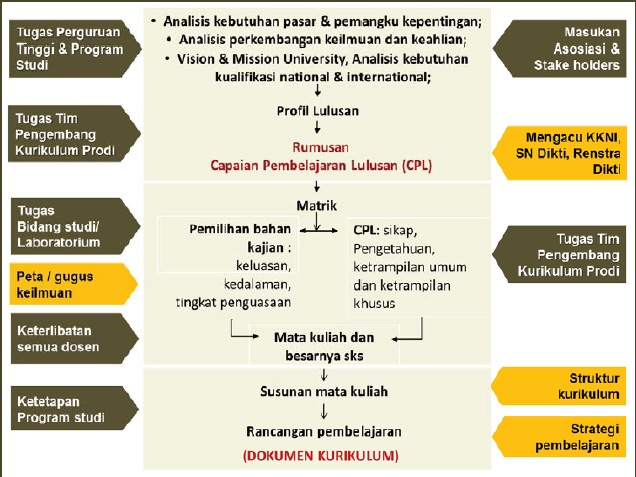
\includegraphics[width=12cm, height=6cm]{Gambar/Penyusunan Kurikulum.jpg}
    \caption{Tahapan Penyusunan Kurikulum}
    \label{fig:gambar1}
\end{figure}

\subsection{Kodifikasi}
Kodifikasi tiap mata kuliah dibuat berdasarkan Peraturan Rektor UNPAR No. III/PRT/2017-03/46 tentang Standar Penyusunan Kurikulum Program Studi di Lingkungan UNPAR. Kode ini terdiri atas 11 dijit, dengan rincian berikut:

\begin{itemize}
    \item 3 digit - kode khas Program Studi: AIF
    \item 2 digit - tahun diberlakukannya kurikulum (2 digit terakhir): 18
    \item 1 digit - urutan tahun pengajaran
    \item 1 digit - nomor urut KBI pengampu mata kuliah
    \item 2 digit - nomor urut mata kuliah per semester, dengan angka pada dijit terakhir sebagai penentu semester; ganjil atau genap
    \item 2 digit - jumlah sks mata kuliah
\end{itemize}

Informasi lengkap terkait kodifikasi ini diberikan di Tabel \ref{fig:gambar2}.

\begin{figure}[H]
    \centering
    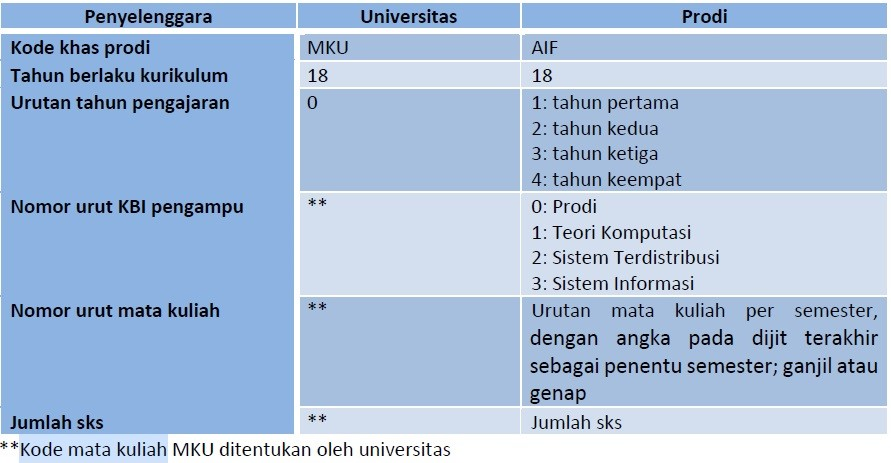
\includegraphics[width=12cm, height=7cm]{Gambar/Kode mata kuliah.jpg}
    \caption{Kodifikasi mata kuliah}
    \label{fig:gambar2}
\end{figure}

\subsection{Bobot Pemrograman}
Berdasarkan hasil evaluasi Kurikulum 2013, salah satu masalah yang ditemukan adalah bahwa mahasiswa masih sulit menguasai materi kuliah di jalur pemrograman, yang merupakan kuliah inti dari Prodi Teknik Informatika UNPAR. Selain karena memang logika pemrograman tidak mudah untuk dipahami, kurangnya pengalaman mahasiswa dalam membangun program komputer juga menjadi penyebab munculnya permasalahan ini.

Selain memperbaiki struktur kuliah jalur pemrograman, dan perbaikan materi perkuliahan, cara lain yang digunakan untuk mendukung kemampuan pemrograman mahasiswa adalah dengan menempatkan bobot pemrograman di kuliah-kuliah yang cocok. Bobot pemrograman ini menentukan di kuliah mana saja mahasiswa harus membangun program komputer, dan seberapa besar skala program komputer yang
dibuat. Bagian pembangunan program komputer misalnya dapat diletakkan pada saat praktikum, atau dijadikan bagian dari tugas kuliah.

Besar bobot pemrograman dalam kurikulum ini adalah 0.25, 0.5, 0.75, dan 1. Penjelasan terkait masing - masing
bobot ini diberikan pada Tabel \ref{fig:gambar3}.

\begin{figure}[H]
    \centering
    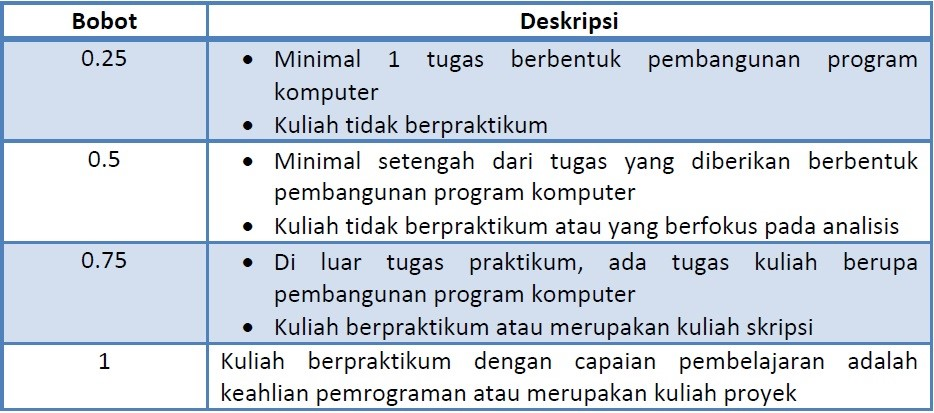
\includegraphics[width=12cm, height=6cm]{Gambar/Bobot Pemorgraman .jpg}
    \caption{Rincian Bobot Pemrograman}
    \label{fig:gambar3}
\end{figure}

\subsection{Struktur Kurikulum}
Berdasarkan hasil evaluasi Kurikulum 2013, struktur kurikulum dibangun dengan mendistribusikan mata kuliah dalam semester - semester. Struktur kurikulum ini terdiri atas 14 sks mata kuliah umum universitas, 100 sks mata kuliah wajib dan pilihan wajib prodi, dan 30 sks kuliah pilihan. Kuliah pilihan mulai diberikan di Semester 4, sedangkan kuliah pilihan wajib diberikan di Semester 6 dan 7. Kuliah pilihan wajib ini terdiri atas 3 mata kuliah, yaitu Proyek Informatika, Proyek Sistem Informasi, dan Proyek Data Science. Pohon Kurikulum 2018 dapat dilihat pada gambar \ref{fig:gambar4}.

\begin{figure}[H]
    \centering
    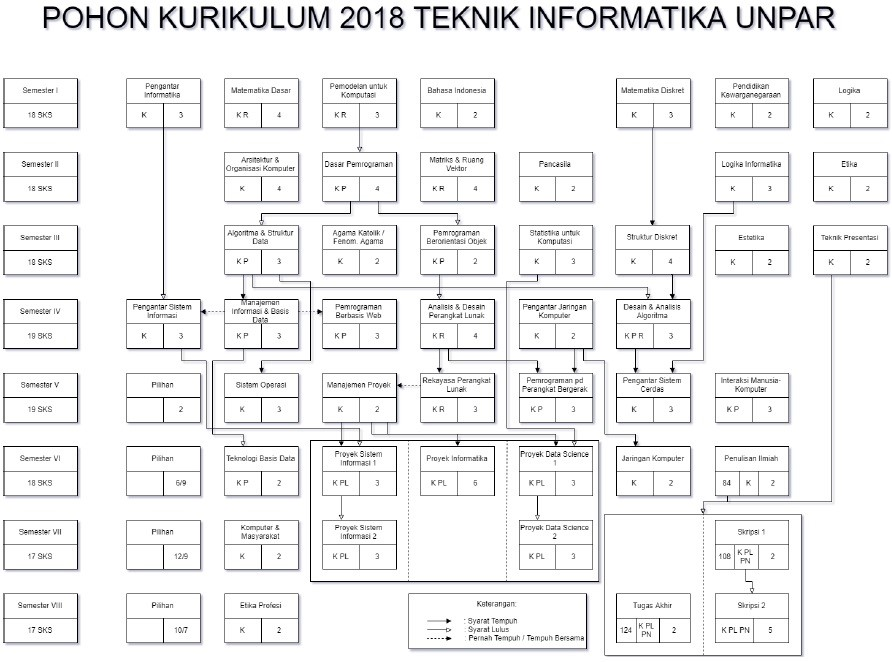
\includegraphics[width=14cm, height=10cm]{Gambar/Pohon Kurikulum .jpg}
    \caption{Pohon kurikulum}
    \label{fig:gambar4}
\end{figure}

Penyusunan struktur kurikulum ini dilakukan dengan memperhatikan hal-hal berikut:

\begin{itemize}
    \item Beban kredit persemester dibatasi maksimum 19 sks.
    \item Capaian pembelajaran yang ingin dicapai pada satu semester harus dapat mendukung capaian pembelajaran yang ingin dicapai di semester berikutnya.
    \item Rangkaian mata kuliah, di mana peletakan mata kuliah dasar dan prasyarat harus tepat sehingga dapat mendukung proses pembelajaran dan pemahaman mata kuliah di tahap selanjutnya. Rangkaian mata kuliah ini diberikan pada Tabel \ref{fig:gambar5}.
\end{itemize}

\begin{figure}[H]
    \centering
    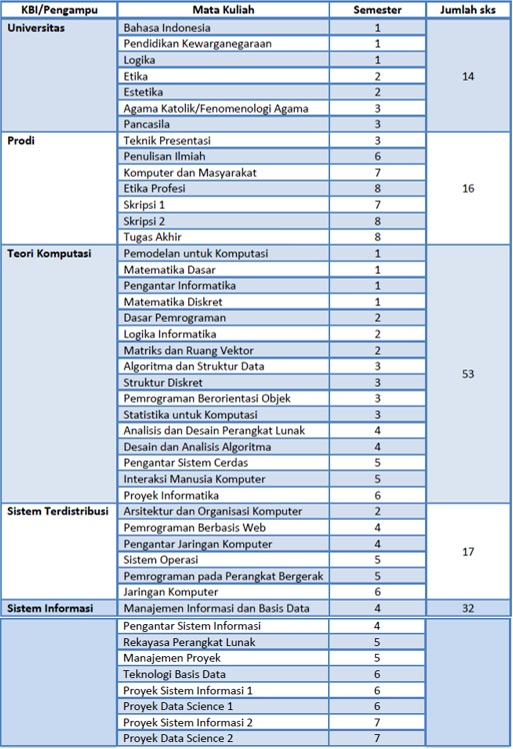
\includegraphics[width=12cm, height=14cm]{Gambar/Mata Kuliah Wajib.jpg}
    \caption{Mata kuliah wajib sesuai bidang keilmuan}
    \label{fig:gambar5}
\end{figure}

Secara umum, terdapat 4 jenis mata kuliah pada Kurikulum 2018, yaitu mata kuliah wajib, pilihan, pilihan wajib, dan sertifikasi. Keempat jenis mata kuliah ini dijelaskan pada bagian-bagian berikutnya. Selain itu, pada kurikulum 2018, diperkenalkan program, di mana masing-masing program terdiri atas banyak mata kuliah pilihan. Dengan cara ini, saat lulus, mahasiswa memiliki titik berat keahlian atau spesialisasi di
bidang ilmu tertentu.

Pada Tabel \ref{fig:gambar7} Semester 7, dapat dilihat bahwa jumlah mata kuliah wajib berkisar antara 2-3 buah dan kuliah pilihan 9-12 buah. Hal ini disebabkan adanya mata kuliah pilihan wajib jalur proyek yang dapat diambil sejak Semester 6. Jika mahasiswa memilih jalur proyek informatika, maka di Semester 7 mata kuliah wajib yang harus diambil adalah 2 buah dengan 12 sks kuliah pilihan. Di kasus ini, mahasiswa dapat mengambil 4 sks kuliah pilihan di Semester 6. Sementara itu, mahasiswa memilih jalur proyek sistem informasi, di Semester 7 mata kuliah wajib yang harus diambil adalah 3 buah dengan 9 sks kuliah pilihan.
Di kasus ini, mahasiswa dapat mengambil 7 sks kuliah pilihan di Semester 6.

\begin{figure}[H]
    \centering
    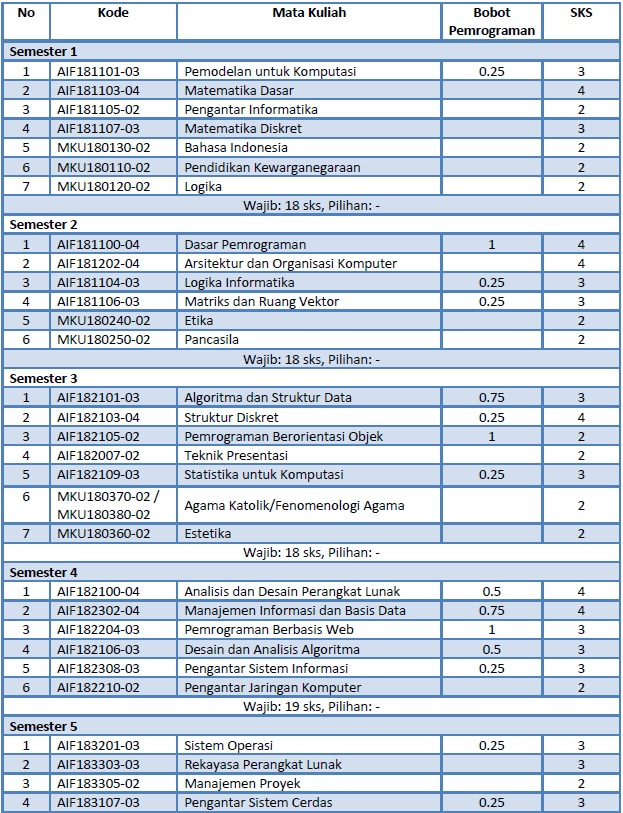
\includegraphics[width=12cm, height=15cm]{Gambar/Struktur Kurikulum 1.jpg}
    \caption{Struktur Kurikulum 2018 (a)}
    \label{fig:gambar6}
\end{figure}

\begin{figure}[H]
    \centering
    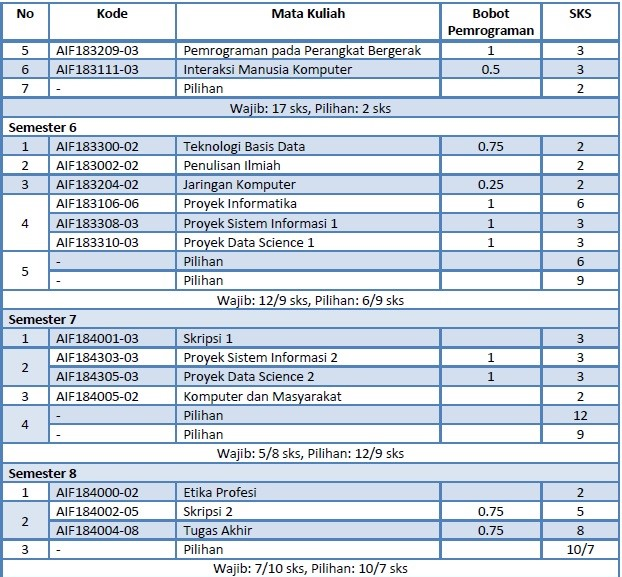
\includegraphics[width=12cm, height=15cm]{Gambar/Struktur Kurikulum 2.jpg}
    \caption{Struktur Kurikulum 2018 (b)}
    \label{fig:gambar7}
\end{figure}

\newpage
\section{Prasyarat Mata Kuliah}
Di Prodi Teknik Informatika terdapat 2 jenis prasyarat, yaitu prasyarat lulus dan prasyarat tempuh. Prasyarat lulus artinya seorang mahasiswa harus lulus mata kuliah prasyarat (nilai minimum D), baru dapat mengambil suatu mata kuliah, sedangkan prasyarat tempuh artinya seorang mahasiswa harus pernah menempuh mata kuliah prasyarat, sebelum dapat mengambil suatu mata kuliah. Rincian prasyarat mata kuliah wajib diberikan pada Tabel \ref{fig:gambar8}, sedangkan rincian prasayarat mata kuliah pilihan diberikan pada Tabel .

\begin{figure}[H]
    \centering
    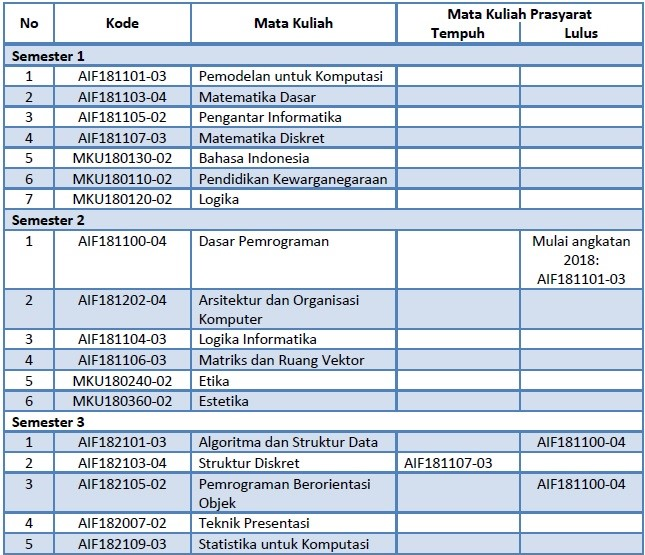
\includegraphics[width=12cm, height=10cm]{Gambar/Prasyarat MK Wajib 1.jpg}
    \caption{Daftar mata kuliah wajib beserta prasyaratnya (a)}
    \label{fig:gambar8}
\end{figure}

\begin{figure}[H]
    \centering
    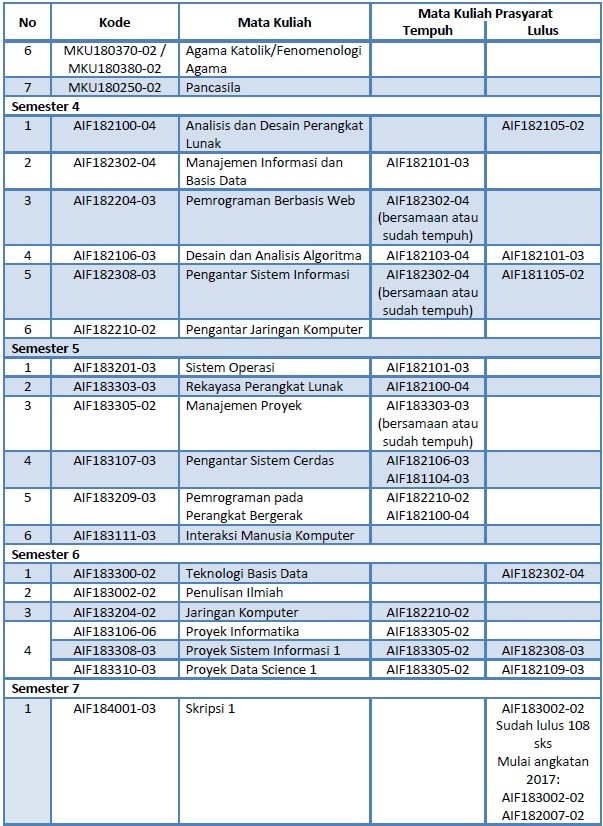
\includegraphics[width=12cm, height=14cm]{Gambar/Prasyarat MK Wajib 2.jpg}
    \caption{Daftar mata kuliah wajib beserta prasyaratnya (b)}
    \label{fig:gambar9}
\end{figure}

\begin{figure}[H]
    \centering
    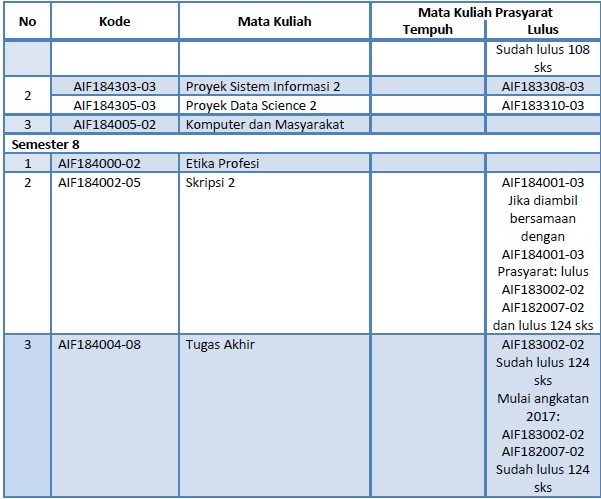
\includegraphics[width=12cm, height=9cm]{Gambar/Prasyarat MK Wajib 3.jpg}
    \caption{Daftar mata kuliah wajib beserta prasyaratnya (c)}
    \label{fig:gambar10}
\end{figure}



\begin{figure}[H]
    \centering
    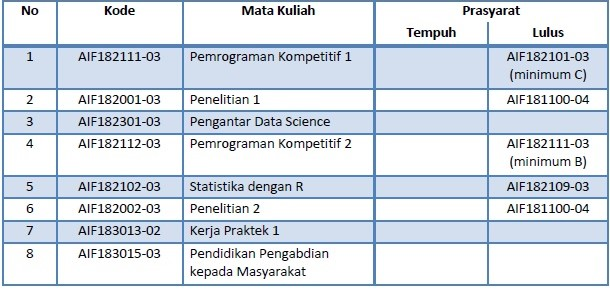
\includegraphics[width=12cm, height=8cm]{Gambar/Prasyarat MK Pilihan 1.jpg}
    \caption{Daftar mata kuliah pilihan beserta prasyaratnya (a)}
    \label{fig:gambar11}
\end{figure}

\begin{figure}[H]
    \centering
    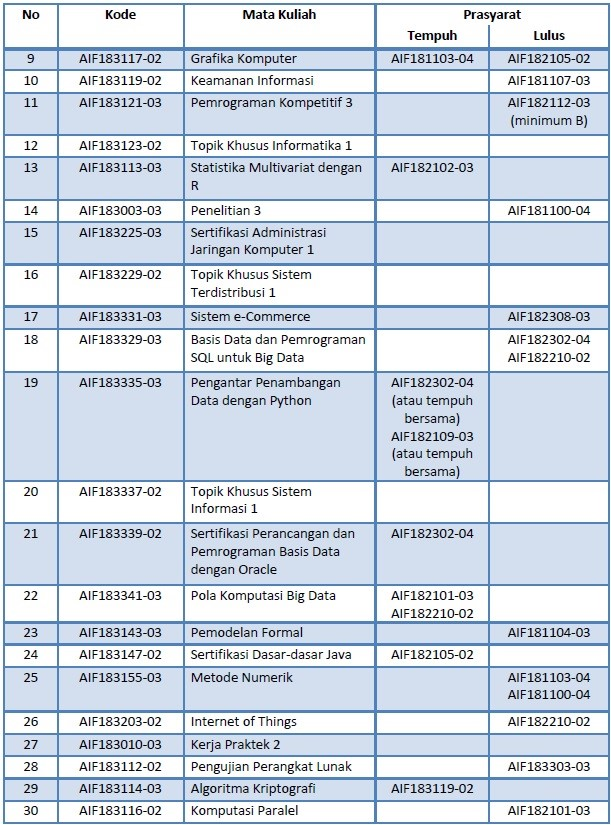
\includegraphics[width=12cm, height=15cm]{Gambar/Prasyarat MK Pilihan 2.jpg}
    \caption{Daftar mata kuliah pilihan beserta prasyaratnya (b)}
    \label{fig:gambar12}
\end{figure}

\begin{figure}[H]
    \centering
    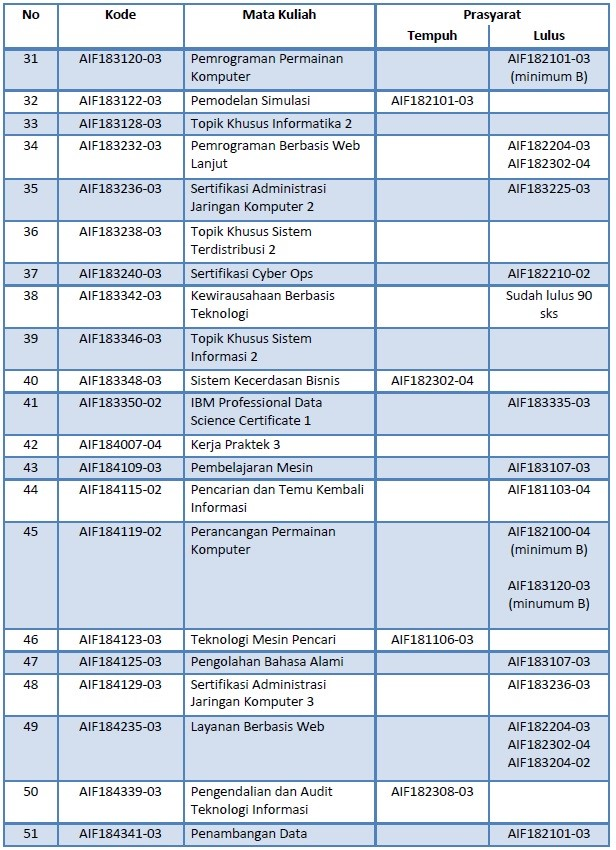
\includegraphics[width=12cm, height=15cm]{Gambar/Prasyarat MK Pilihan 3.jpg}
    \caption{Daftar mata kuliah pilihan beserta prasyaratnya (c)}
    \label{fig:gambar13}
\end{figure}

\begin{figure}[H]
    \centering
    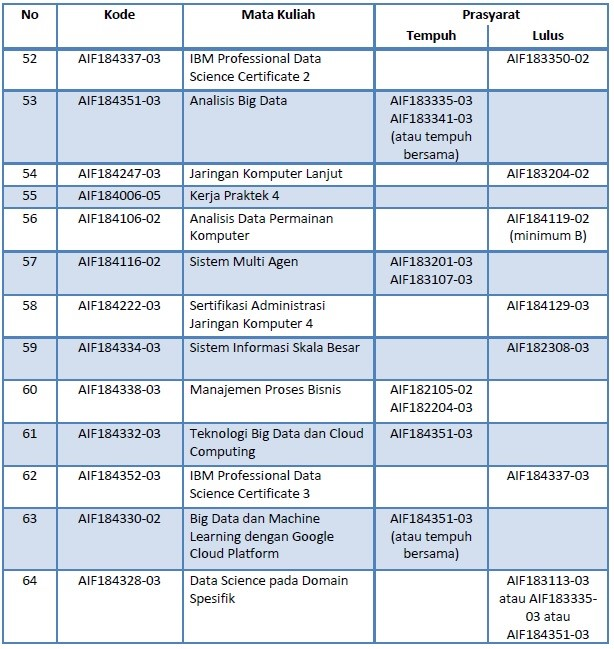
\includegraphics[width=12cm, height=12cm]{Gambar/Prasyarat MK Pilihan 4.jpg}
    \caption{Daftar mata kuliah pilihan beserta prasyaratnya (d)}
    \label{fig:gambar14}
\end{figure}

\newpage
\section{Electron}
\textit{Electron} adalah sebuah kerangka kerja untuk mengembangkan aplikasi \textit{desktop} asli lintas platform menggunakan teknologi web seperti \textit{JavaScript}, \textit{HTML}, dan \textit{CSS}. Dengan menggunakan \textit{electron} pengembang web yang terampil dapat mengembangkan aplikasi lintas platform semacam itu tanpa perlu keahlian khusus sistem operasi yang lain. Keunggulan dari kerangka kerja \textit{electron} adalah bersifat \textit{Open Source}, dipelihara di \textit{Github} oleh komunitas dan bersifat \textit{Cross Platform}, bisa dijalankan di \textit{Mac}, \textit{Windows} dan \textit{Linux}. Aplikasi-aplikasi yang dibuat menggunakan \textit{electron} seperti \textit{Atom Editor}, \textit{Visual Studio}, \textit{Wordpress.com (Desktop Version)}, \textit{Avocode} dan sebagainya.

\textit{Electron} menggabungkan \textit{browser web} yang lengkap: \textit{chromium}, versi \textit{open source Google Chrome}. Ini dibundel bersama dengan instruksi spesifik platform untuk memastikan bahwa segala sesuatu berperilaku tepat seperti yang diharapkan pengembang di semua sistem. Itu sebabnya versi desktop \textit{slack} membutuhkan lebih dari 200MB ruang \textit{hard drive} dengan sebagian besar \textit{chrome} ada di dalamnya. Maka dari itu kelemahan dari kerangka kerja \textit{electron} adalah boros \textit{memory} dan memakan waktu yang sedikit lebih lama untuk menjalankannya, karena setiap aplikasi \textit{electron} mengunduh bundel sebagian besar \textit{chromium}, dan setiap aplikasi yang dijalankan mengeksekusi potongan kode yang baik. Tidak ada pembagian sumber daya di sini seperti yang ada dengan aplikasi asli, yang berarti aplikasi \textit{electron} akan mengambil lebih banyak ruang dan memori \textit{hard drive} daripada aplikasi yang dikembangkan dengan platform kita secara khusus.

Aplikasi yang dibangun dengan \textit{electron} terdiri dari dua jenis proses, yaitu proses utama dan beberapa proses  \textit{renderer} dengan mengikuti pola \textit{master-slave}. Proses utama aplikasi adalah \textit{master} dan beberapa proses renderer adalah budak yang berkomunikasi menggunakan \textit{Inter-Process Communication} (IPC). Gambar \ref{fig:gambar15} menunjukkan bahwa ini serupa dengan \textit{browser Chromium} yang memiliki satu jendela utama dan banyak tab (proses renderer).

\begin{figure}[H]
    \centering
    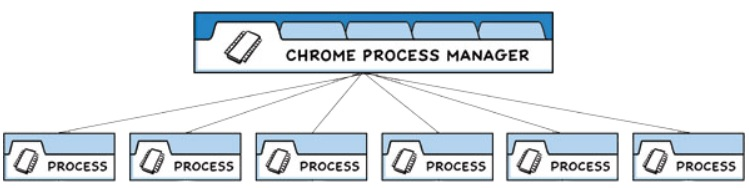
\includegraphics[width=12cm, height=6cm]{Gambar/Rendered Processes.jpg}
    \caption{Sebuah proses utama dengan beberapa proses \textit{renderer}. Proses ini mirip dengan jendela \textit{browser chromium} dengan banyak tab}
    \label{fig:gambar15}
\end{figure}

Secara khusus, electron akan melihat masukan awal di manifes package.json yang dimasukkan ke dalam proyek untuk menentukan titik masuk aplikasi yang dijalankan sebagai prosess utama.

Proses utama bertanggung jawab untuk merespons peristiwa siklus hidup aplikasi seperti \textit{starting up}, \textit{quiting}, \textit{preparing to quit}, \textit{going to the background}, \textit{coming to the foreground} dan sebagainya. Proses utama juga bertanggung jawab untuk berkomunikasi dengan API sistem operasi asli. Misalnya untuk menampilkan dialog untuk membuka atau menyimpan \textit{file}. Proses utama juga dapat membuat dan menghancurkan proses \textit{renderer} menggunakan modul \textit{BrowserWindow} \textit{electron}.

Proses renderer dapat memuat halaman web untuk menampilkan \textit{GUI}. Setiap proses memanfaatkan arsitektur multi-process chromium dan berjalan di threadnya sendiri. Tidak seperti laman web biasa, ada akses ke semua Node APIs dalam proses renderer, yang memungkinkan developers memanfaatkan modul asli dan tingkat interaksi sistem yang lebih rendah. 

Untuk cara membuat aplikasi dengan \textit{electron} adalah sebagai berikut :

\begin{enumerate}
    \item Install terlebih dahulu Node.js dan npm (pakai versi terakhir LTS yang tersedia).
    \item Cek versinya dengan mengetik node -v dan npm -v pada command prompt.
    \item Buat folder dan inisialisasi paket npm dengan mengetik mkdir namaFolder lalu ketik cd namaFolder setelah itu ketik npm init pada \textit{command prompt}. Maka isi package.json akan seperti pada gambar \ref{fig:gambarJson}.
    
    \begin{figure}[H]
        \centering
        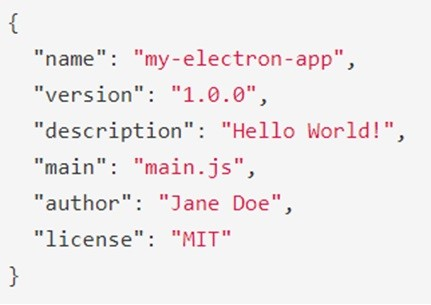
\includegraphics[width=12cm, height=6cm]{Gambar/Package Json.jpg}
        \caption{Package.json}
        \label{fig:gambarJson}
    \end{figure}
    \item Install aplikasi \textit{electron} ke dalam folder yang telah dibuat dengan cara mengetik npm install --save-dev electron pada command prompt.
    \item Pada \textit{script file} package.json tambahkan \textit{command start} seperti pada gambar \ref{fig:startCommand}.
    
    \begin{figure}[H]
        \centering
        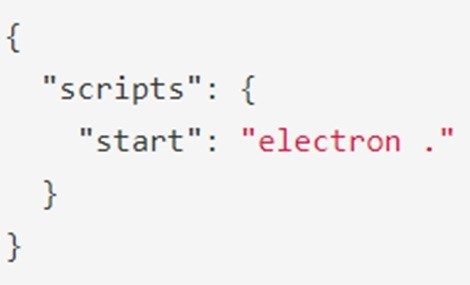
\includegraphics[width=12cm, height=6cm]{Gambar/json file.jpg}
        \caption{Start command}
        \label{fig:startCommand}
    \end{figure}
    \item Jalankan aplikasi \textit{electron} dengan mengetik npm start pada command prompt.
\end{enumerate}





\section{Vis.Js}

\subsection{Timeline}

\subsection{Network}

\section{Github}
Github adalah layanan \textit{hos web} bersama untuk proyek pengembangan perangkat lunak yang menggunakan sistem kendali versi Git dan layanan \textit{hosting} internet secara gratis. Github berfungsi sebagai manajemen proyek dengan sistem \textit{versioning code} yang digunakan untuk developer dalam bekerja bersama-sama dengan rekan, merencanakan proyek, dan melacak pekerjaan. Selain berfungsi untuk menyimpan repositori dan alat kolaborasi proyek, Github juga bisa sebagai sarana dalam mendapatkan pekerjaan. Ada banyak \textit{programmer} yang mengajak \textit{programmer} sesama pengguna Github untuk bekerjasama dalam mengerjakan suatu proyek. Hal ini bisa terjadi karena di Github memiliki halaman profil yang berisi data pribadi seperti foto, email, jumlah repositori yang dimiliki dan jumlah \textit{follower} (semakin banyak akan menjadi pertimbangan bagi programmer lain untuk merekrut). Di Github dapat diatur status proyek menggunakan fitur \textit{public} atau \textit{private}. Jika \textit{public} artinya project dapat dilihat, diubah, dan diunduh oleh siapa saja. Jika \textit{private} artinya project hanya bisa dilihat, diubah dan diunduh oleh pemilik dan tim project yang \textit{diinvite} pada project, tetapi fitur \textit{private} dibatasi hanya untuk tiga kontributor, jika ingin lebih dari tiga maka diharuskan untuk \textit{upgrade} ke Github versi berbayar (GitHub Pro). Untuk Cara menggunakan Github adalah seperti berikut :

\begin{enumerate}
    \item Login
    
    Sebelum mulai untuk menggunakan Github pastikan bahwa kita sudah login ke website Github terlebih dahulu, jika belum memiliki akun sebaiknya membuat akun terlebih dahulu. Saat membuat akun, kita akan diminta untuk mengisi beberapa data pribadi seperti nama dan alamat email, kemudian akan diminta untuk melakukan verifikasi secara langsung.
    \item Membuat repositori
    
    Setelah masuk ke akun Github, kita bisa langsung mulai untuk membuat repositori. Caranya dengan mengklik tombol New yang terdapat pada menu repositori, selanjutnya kita akan diarahkan untuk menuju halaman pembuatan repositori. Membuat repositori baru tentu membutuhkan beberapa informasi awal seperti nama repositori, deskripsi yang berfungsi untuk memberi penjelasan terkait repositori yang kita buat, jenis repositori yang terdiri dari \textit{public} atau \textit{private}. Pengaturan yang bersifat publik tentu bisa membuat orang lain mengakses repositori yang kita buat, sebaliknya jika tidak ingin ada orang lain yang melakukan akses terhadap repositori milik kita maka gunakan pengaturan private. Jika ketiga data tersebut sudah terpenuhi, kita bisa melanjutkan dengan mengklik \textit{create repository}.
    \item Membuat \textit{local} folder
    
    Membuat folder lokal yang terdapat pada komputer tentu berfungsi untuk melakukan penyimpanan \textit{update file} dari repositori yang dibuat ketika terjadi perubahan tertentu, saat folder tersebut berhasil dibuat kita bisa membuka folder tersebut kemudian klik kanan untuk memilih menu Git Bash Here. Sehingga folder tersebut akan berubah menjadi repositori.
    \item Memasukkan file ke repositori
    
    Untuk dapat menambahkan dan memasukkan file ke repositori yang sudah dibuat, kita bisa membuat file di dalam folder tersebut kemudian dilanjutkan dengan membuka bagian Git Bash sesuai perintah.
    \item Membuat commit
    
    Fitur commit berfungsi untuk menambahkan \textit{update file} dan komentar, juga membantu rekan tim yang ada untuk mengkonfirmasi \textit{update file} di proyek yang sedang dikerjakan.
    \item \textit{Remote repository}
    
    Kita dapat mengupload file yang sudah dibuat di \textit{local disk} dengan menggunakan \textit{remote repository}.
    \item Melakukan push ke github
    
    Kita dapat melakukan \textit{push} yang berfungsi untuk mengunggah hasil akhir dari pekerjaan kita, setelah itu kita bisa melakukan pengecekan pada repositori untuk memastikan bahwa file-file yang ditambahkan sudah masuk dan sesuai dengan yang diinginkan.
    \item Melakukan pull dari github
    
    Saat kita ingin melanjutkan pekerjaan kita, sebaiknya kita melakukan \textit{pull} terlebih dahulu yang berfungsi agar file pekerjaan yang terdapat di \textit{local folder} sudah diperbaharui dengan hasil pekerjaan tim kita.
\end{enumerate}

Github menggunakan sistem pengontrol versi yang disebut dengan Git. Git adalah salah satu sistem pengontrol versi (\textit{Version Control System}) pada proyek perangkat lunak yang diciptakan oleh Linus Torvalds pada tahun 2005. Software ini bersifat open source dan bisa di-download untuk \textit{Linux}, \textit{Windows}, \textit{Solaris} dan \textit{Mac}. Terdapat beberapa perintah dasar Git yang sering digunakan dalam pengerjaan proyek, seperti berikut :

\begin{enumerate}
    \item git config
    
    berfungsi untuk mengatur konfigurasi tertentu sesuai keinginan kita, seperti : e-mail, username, format file, dan sebagainya. 
    
    Contoh perintah untuk mengatur email : 
    git config --global user.email yourEmail
    
    \item git init
    
    berfungsi untuk membuat \textit{repositori} baru.
    
    Caranya : git init
    \item git add
    
    berfungsi untuk menambahkan file ke index.
    
    Contoh perintah untuk menambahkan file bernama temp.txt yang ada di direktori lokal ke index : git add temp.txt
    \item git clone 
    
    berfungsi untuk membuat salinan repositori lokal.
    
    Contoh perientah untuk membuat salinan kerja dari server : git clone username@host:/path/to/repository
    \item git commit
    
    berfungsi untuk melakukan \textit{commit} perubahan ke head, perintah ini dilakukan sebelum melakukan perintah \textit{push}.
    
    Contoh perintah untuk melakukan \textit{commit} : git commit –m "Keterangan \textit{commit}"
    \item git push
    
    berfungsi untuk mengirimkan perubahan ke \textit{remote} repositori.
    
    Contoh perintah untuk melakukan \textit{push} : git push
    \item git pull
    
    berfungsi untuk menggabungkan semua perubahan yang ada di \textit{remote} repositori ke direktori lokal.
    
    Contoh perintah untuk melakukan \textit{pull} : git pull
    \item git branch
    
    berfungsi untuk untuk me-list, membuat atau menghapus \textit{branch}.
    
    Contoh perintah untuk menampilkan semua branch yang ada di repositori : git branch
    \item git checkout
    
    berfungsi untuk membuat branch atau untuk berpindah diantaranya.
    
    Contoh perintah untuk membuat branch baru : git checkout -b <branch-name>
    
    Contoh perintah untuk berpindah dari branch satu ke lainnya : git checkout <branch-name>
    \item git merge
    
    berfungsi untuk menggabungkan sebuah branch ke branch aktif.
    
    Contoh perintah untuk melakukan \textit{merge} : git merge
    \item git fetch
    
    berfungsi untuk menampilkan semua objek dari \textit{remote repository} yang tidak berada di direktori kerja lokal.
    
    Contoh perintah untuk melakukan fetch : git fetch origin
    \item git revert
    
    berfungsi untuk membatalkan \textit{commit} yang ada.
    
    Contoh perintah untuk melakukan \textit{revert} : git revert "commit number"
\end{enumerate}
\textit{Version control system} adalah sistem yang mencatat semua perubahan yang dilakukan pada file sehingga semua riwayatnya akan terekam dan bisa dilihat kembali nanti. Saat developer membuat proyek baru, mereka selalu pembaharuan terhadap kodenya. Bahkan, setelah proyeknya online, developer tetap harus memperbarui versinya, memperbaiki bug, menambahkan fitur baru, dan lain sebagainya. Version control system membantu developer melacak perubahan yang mereka lakukan terhadap basis kode. Tak hanya itu, sistem ini juga mencatat siapa saja yang membuat perubahan serta memulihkan kode yang telah dihapus atau dimodifikasi. Dengan menggunakan sistem tersebut, maka tidak ada kode yang saling tertimpa. 






